\section{L'implementazione del database}
Nelle sezioni precedenti si è discusso delle proprietà
offerte dai diversi tipi di database e
delle necessità che il dominio impone sul sistema.
La scelta del database deriva quindi dall'incrocio di tutte queste condizioni,
individuando la tecnologia che meglio riesce a rispondere alle esigenze del progetto.
Ogni tipologia di database comporta un approccio differente alle informazioni,
implicando una strategia di salvataggio e manipolazione dei dati propria.
Le strutture che modellano le entità devono quindi
essere create per sfruttare nella maniera più efficiente possibile
i vantaggi offerti dalla tecnologia scelta.\\
\\
Una volta scelto il database e le strutture in base alla modalità
che più si addicono alle esigenze del progetto,
l'utilizzo di servizi in cloud comporta una maggiore attenzione anche
alle proprietà legate al mantenimento del servizio,
dalle quali derivano le proprietà di scalabilità e affidabilità.
La grande differenza tra i vari servizi sta nelle proprietà del server
incaricato di fornire il potere computazionale necessario per l’esecuzione.
L’architettura del server e la sua integrazione con la tecnologia del database
determinano infatti l’effettiva capacità di scalabilità del servizio.\\
\\
Si intende scalabilità verticale la capacità di aumentare le risorse
della stessa macchina in cui si esegue il codice.
La scalabilità verticale viene definita nel momento di creazione del servizio,
in cui si determinano le risorse da dedicare alla macchina che esegue il programma.
Trattandosi di macchine virtualizzate,
è sempre possibile in un secondo momento aumentare le prestazioni in caso di necessità.\\
\\
Per scalabilità orizzontale si intende invece la capacità di
delegare il carico di lavoro su più macchine, eventualmente coordinando le modifiche.
Questo permette una risposta alle richieste più resistente,
riducendo il rischio di colli di bottiglia che potrebbero venirsi a formare nell’utilizzo di un nodo singolo.
La scalabilità orizzontale richiede però l'implementazione
di tecnologie apposite integrate con il database che permettano l'esecuzione in nodi fisici differenti. \\
\\
Una volta individuata la tecnologia adatta e il livello di scalabilità desiderati,
è bene considerare le altre necessità o le opportunità aggiuntive generate
dalla presenza di un database nel progetto. \\
\\
L’alta disponibilità(HA) è la proprietà di garantire l’accesso al servizio nonostante i guasti.
Ad esempio, si può mantenere una macchina identica al server principale in grado di replicare il servizio,
spostando il carico in caso di guasto del server principale.
Si misura in “numero di nove”, ovvero la quantità di nove presenti
nella percentuale del tempo per il quale si garantisce la disponibilità del servizio.
I servizi offrono diverse qualità di HA, in base alle funzionalità desiderate.\\
\\
Alcuni servizi possono presentare offerte di backup
per riportare il server nello stesso stato di qualche momento precedente.
Questo permette il ripristino del sistema a un punto precedente
rispetto all'avvenimento di eventuali errori o guasti del sistema.\\
\subsection{La scelta del database}

Viste le necessità del progetto in ambito di scalabilità
e le caratteristiche del dominio,
si individua nei database documentali la tecnologia più adatta
per gestire la persistenza centrale dell'applicazione.\\
\\
I database documentali, facenti parte della categoria dei database non relazionali,
rappresentano un paradigma di gestione dei dati
che organizza le informazioni in documenti.
Ogni documento è un'unità autonoma che incapsula la descrizione di un'entità,
contenendo le sue proprietà.
Tali documenti sono logicamente raggruppati in collezioni.
All'interno di una collezione,
ciascun documento è univocamente identificato da un proprio identificativo,
garantendo l'accesso diretto e la manipolazione individuale.\\
\\
Un aspetto distintivo e strategicamente rilevante dei database documentali è
la loro intrinseca capacità di supportare la scalabilità orizzontale in modo nativo.
Data la natura dei documenti e il loro accoppiamento debole con gli altri elementi,
la separazione delle collezioni risulta particolarmente semplificata,
favorendo un partizionamento dei dati,  
essenziale per distribuire il database su diversi nodi fisici di archiviazione.
Questo vantaggio è fondamentale in architetture distribuite e ambienti ad alta intensità di dati.\\
\\
Un altro vantaggio derivato dall'utilizzo di un database non relazionale
è la propensione verso la denormalizzazione degli elementi del dominio, 
sia strutturale che logica.
La denormalizzazione consiste nel riportare le stesse proprietà degli elementi in più collezioni, 
riducendo così, se correttamente ottimizzata, 
il numero di join o richieste al database necessario per soddisfare le richieste.
Infatti, vista la riduzione di efficienza nell'incrocio tra entità, 
dovuta a una difficoltà intrinseca nell'ottimizzare le join tra documenti,
si propende, invece che a incrociare i dati, a duplicarli sui i vari documenti.
Le operazioni di join sono così agevolate,
in quanto possono essere ottimizzate per 
far risiedere la risorsa voluta all'interno dello stesso documento o nella stessa partizione dell'elemento di partenza, 
minimizzando la necessità di operazioni di giunzione di tabelle o di lettura tra nodi distinti.
Questo permette di aggregare i dati attorno agli elementi chiave su cui vertono le richieste,
favorendo la divisione dei dati anche in caso di relazioni complesse.\\
\\
La denormalizzazione comporta però intrinsecamente
alcune sfide a livello di consistenza dei dati,
in particolare per le operazioni di modifica che coinvolgono informazioni duplicate.
Infatti, pur se si modificasse atomicamente il documento direttamente coinvolto dalla modifica,
bisognerebbe comunque aggiornare tutte le altre parti che includono quella proprietà.
Oltre a dover progettare l'applicazione affinché sia resiliente all'inconsistenza temporanea,
ad esempio mostrando dati "vecchi" per un breve periodo prima che le modifiche vengano propagate, 
o implementando logiche di compensazione che possano correggere eventuali discrepanze,
è quindi necessario implementare la logica per garantire che la modifica venga propagata correttamente.
Esistono diverse strategie gestire le informazioni duplicate in modo efficace e mitigarne l'impatto. 
Una delle soluzioni avviene tramite trigger a livello di database, 
che scatena la chiamata che corregge poi i dati ove necessario.
Le code di messaggistica prevedono invece un orchestratore per la distribuzione degli aggiornamenti, 
che riceve notifiche delle variazioni e le elabora per poi applicare le modifiche.
Un'altra tecnica è l'applicazione di servizi in background che periodicamente scansionano e sincronizzano i dati. 
Infine, si possono adottare timestamp o numeri di versione su ciascun documento o campo denormalizzato,
permettendo alle applicazioni di determinare la versione più recente di un dato, 
risolvendo i conflitti quando si presentano aggiornamenti concorrenti o ritardati.\\
\\
Implementando automaticamente e nativamente la scalabilità orizzontale,
il database relazionale ci permette quindi di gestire con efficienza
l'incremento dei volumi di dati e dei carichi di lavoro senza interventi complessi.
Fornisce inoltre un supporto diretto all'esigenza dell'architettura
riguardo alla necessita di letture performanti
da entrambi i lati di relazioni molti-a-molti:
attraverso il partizionamento strategico,
i dati correlati possono essere collocati in partizioni vicine
per ottimizzare le letture da entrambi i lati della relazione.
Infine, un'attenta progettazione del modello di dati,
che include una denormalizzazione strategica e l'utilizzo degli indici,
garantirà un tempo di recupero ridotto per le informazioni,
massimizzando la reattività del sistema e l'efficienza complessiva.\\
\\
Un confronto con il paradigma relazionale evidenzia le ragioni della sua esclusione per le esigenze del nostro progetto.
Sebbene i database relazionali siano soluzioni consolidate per la gestione di dati strutturati,
presentano delle limitazioni che non si allineano con i requisiti di scalabilità richiesti.
La necessità di controllare le transazioni al fine di garantire le proprietà ACID
influenza il numero massimo di connessioni contemporanee che possono gestire,
limitando la capacità di rispondere a un numero massiccio di richieste simultanee.
Inoltre la loro architettura non prevede una separazione fisica di schemi in relazione tra loro,
legandole alla stessa partizione logica.
Questo impone intrinsecamente dei vincoli sulla scalabilità orizzontale,
in quanto l'implementazione dello sharding, sebbene possibile,
viene lasciata interamente a carico dello sviluppatore,
introducendo un significativo onere di progettazione, sviluppo e manutenzione.\\
\\
La gestione di relazioni molti-a-molti nel modello relazionale 
si pone infatti in diretto contrasto con la denormalizzazione dei dati,
utilizzando un'unica tabella di giunzione per descriverne il rapporto.
Se si provasse a dividere in partizioni gli schemi relazionali,
dalla distribuzione della tabella di giunzione ne conseguirebbe uno svantaggio,
indipendentemente dalla strategia usata.
Separando la tabella in base a un elemento si andrebbe infatti a compromettere
l'abilità di ritrovare i dati in base all'altro elemento e viceversa:
per quanto si avrebbero tutti i dati di un elemento dell'associazione sulla sua stessa partizione,
sfruttando al massimo la velocità di unione tra schemi dei relazionali,
per eseguire la ricerca in senso inverso bisognerebbe invece 
allargare la richiesta a tutte le partizioni del sistema.
In un ambiente distribuito e con volumi di dati in crescita,
le join richiedono quindi l'analisi e il trasferimento di grandi quantità di dati tra nodi diversi,
riducendo le performance complessive.
Questi fattori combinati ci hanno portato a escludere il modello relazionale.\\
\\
Essendo il progetto già improntato sulla piattaforma Azure,
la ricerca verte inizialmente tra le opzioni che mette a disposizione.
Azure offre un’ampia scelta di database documentali che possono essere integrati con il resto dell’ecosistema.
Tuttavia, Azure presenta un servizio completamente gestito e nativo
per i database non relazionali chiamato Azure Cosmos DB.
Garantendo la massima interoperabilità all'interno dell'ecosistema,
si procede analizzando le proprietà e i vantaggi offerti da Cosmos DB.\\
\\
Azure Cosmos DB si distingue per la sua capacità di scalare orizzontalmente in maniera illimitata,
consentendo di gestire volumi di dati e carichi di lavoro molto elevati,
fino a milioni di richieste al secondo,
grazie alla possibilità di distribuire il carico su più regioni Azure.
È stato infatti ideato per presentare un'architettura distribuita,
con replica automatica dei dati,
assicurando un'elevatissima disponibilità e resilienza.
Queste vengono assicurate anche in caso di interruzioni regionali,
grazie a meccanismi di failover automatico.
Inoltre, la distribuzione globale garantisce che i dati siano sempre vicini agli utenti,
riducendo drasticamente la latenza a millisecondi
(con SLA del 99.999\% di disponibilità per account multi-regione).
Consente l'indicizzazione attraverso più partizioni in maniera
automatica e personalizzabile ottimizzando le query,
riducendo la complessità e migliorando le prestazioni,
senza richiedere oneri di gestione manuale degli indici.\\
\begin{figure}[h!]
    \centering
    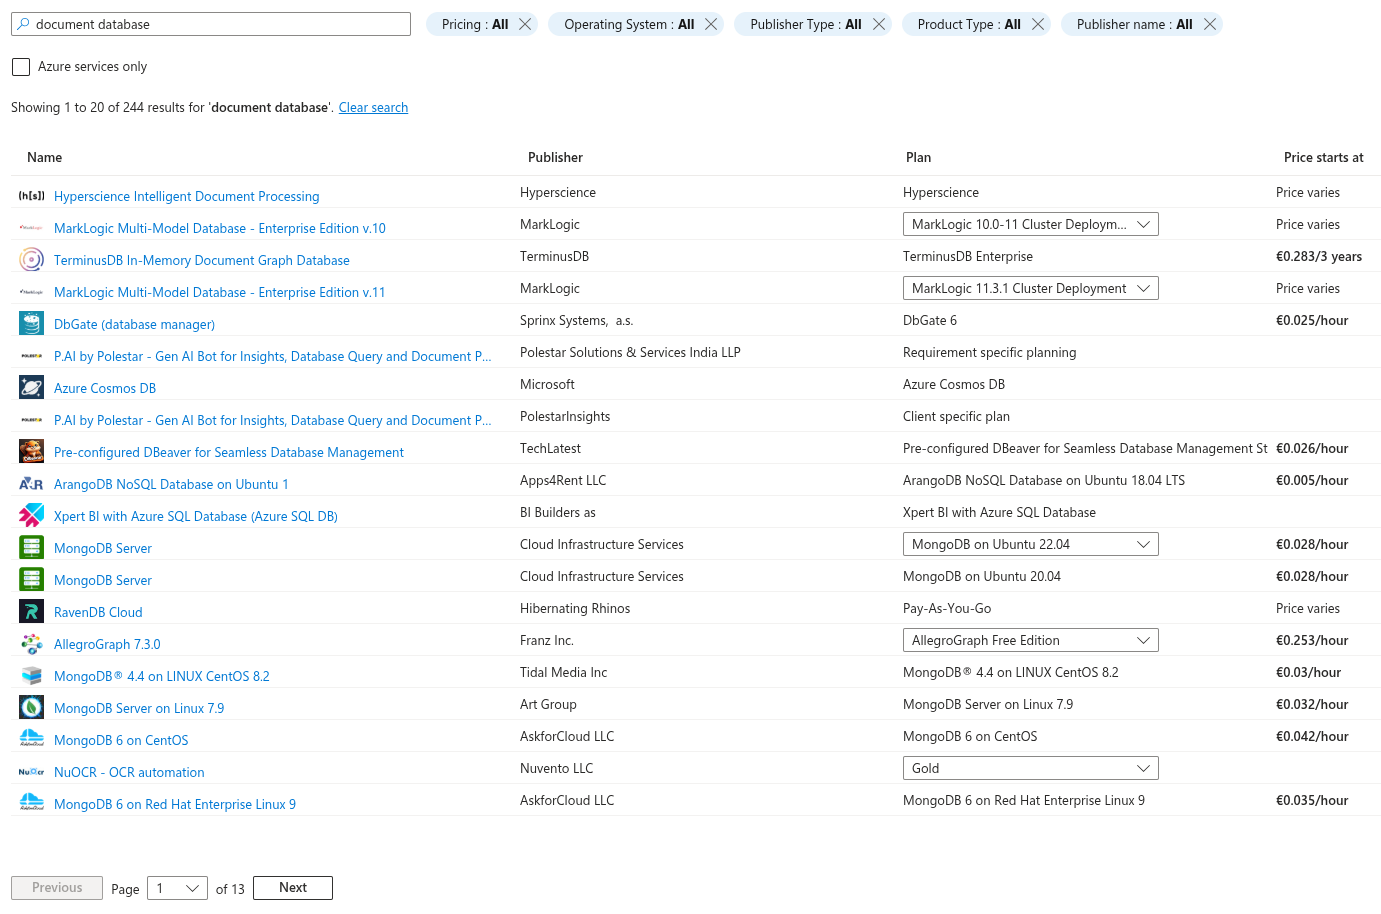
\includegraphics[width=\textwidth]{AzureDatabase.png}
    \caption{Proposte di Azure per i database documentali}
\end{figure}


\begin{wrapfigure}{r}{0.25\textwidth}
    \centering
    
\includegraphics[height=.12\textheight]{cosmos.png}
    Azure Cosmos
\end{wrapfigure}
Pur essendo focalizzato sui database documentali,
Cosmos DB è però una soluzione multi-modello e multi-API.
Supporta infatti, oltre alla sua API nativa per NoSQL (che usa il modello a documenti JSON),
anche API compatibili con MongoDB, Apache Cassandra, Apache Gremlin (per i grafi) e Azure Table.
Questa versatilità permette agli sviluppatori di utilizzare strumenti familiari,
semplificando la migrazione di applicazioni esistenti o
lo sviluppo di nuove con la flessibilità di scegliere il modello di dati più appropriato.\\
\\
A livello di costi è difficile portare un'analisi precisa,
in quanto tutti i competitor presentano servizi
con capacità, disponibilità e intregrazione differenti.
I modelli di pagamento che utilizzano metriche di utilizzo diverse,
rendendo necessarie ulteriori analisi che dipendono anche
dall'effettiva tipologia e quantità delle richieste che vertono sul database.
Di seguito viene riportata una tabella per comparazione i costi delle alternative principali.
Cosmos usa come metrica le Rerquest Units(RU) per quantificare l'impatto di una richiesta sul database.
Le RU rappresentano un'astrazione delle risorse di sistema (CPU, I/O, memoria).
Ogni operazione consuma RU, proporzionalmente alla sua
complessità, dimensione e al carico computazionale richiesto.\\

\begin{longtable}{|P{3.2cm}|P{4.2cm}|P{4.2cm}|P{3cm}|}
    \hline
    \textbf{Servizio}      & \textbf{Costo ogni milione di scritture}\newline(normalizzate a 1 KB) & \textbf{Costo ogni milione di scritture}\newline (normalizzate a 1 KB) & \textbf{Costo di manutenzione GB/mese} \\
    \hline
    \endhead
    AWS DynamoDB           & \$1.25                                                                & \$0.25                                                                 & \$0.25                                 \\
    \hline
    Google Cloud Firestore & \$0.90                                                                & \$0.30                                                                 & \$0.156                                \\
    \hline
    Azure Cosmos DB        & In base al consumo di RU, \$5.84 al mese ogni 100RU/s                 & In base al consumo di RU, \$5.84 al mese ogni 100RU/s                  & \$0.25 (Transazionale)                 \\
    \hline
    \caption{Costi dei principali database documentali gestiti in Cloud}
\end{longtable}

La difficoltà di stabilirne il costo in una fase iniziale
è mitigata però dalla presenza di un piano gratuito perenne.
Cosmos DB offre infatti una quota gratuita di risorse iniziali,
per tutta la durata dell'utilizzo.
Il piano prevede 25 GigaByte di memoria gratuita,
a cui si aggiungono 1000 RU/s offerti per ogni categoria di operazione, 
suddivise in lettura, scrittura e eliminazione. 
Dato lo stadio iniziale del progetto queste caratteristiche sono state considerate sufficenti,
permettendo di sfruttare e testare le capacità di distribuzione.
Nel caso in cui, sfruttando dati derivati dall'utilizzo effettivo dell'applicazione,
un'analisi condotta durante fasi successive del progetto faccia emergere che 
Cosmos DB non rappresenti l’opzione più adeguata, 
lo spostamento dei dati verso un altro gestore comporterà uno sforzo limitato,
data la compatibilità nella rappresentazione dei dati tra le diverse tecnologie di database documentali.

\subsection{La configurazione di Cosmos DB}

La creazione di una nuova istanza di Cosmos DB
richiede la definizione delle impostazioni di funzionamento,
che ne determinano le proprietà, a livello di disponibilità, ridondanza, sicurezza e resilienza ai guasti.\\
\\
La prima impostazione riguarda la distribuzione geografica dei dati.
Cosmos distribuisce sue risorse in zone, che vengono raggruppate in regioni.
L'opzione di usare delle availability zones duplica i dati su più zone all'interno della stessa regione.
Questo crea ridondanza dei dati per una maggiore resistenza ai guasti,
e così facendo aumenta la disponibilità dei dati, 
che da un disponibilità garantita iniziale per la zona singola del 99.99\% (sulle scritture) sale al 99.995\%,
evitando la perdita dei dati e delle funzionalità in caso una zona non sia più raggiungibile.
L'aggiunta di ulteriori regioni diminuirebbe il rischio indisponibilità a causa di guasti
(i dati verrebbero duplicati anche tra le varie regioni),
ma aumenterebbe la complessità e il costo dell'applicazione.
Per una fase iniziale si è optato per garantire una ridondanza a livello di zone,
selezionando quindi l'opzione delle availability zones, 
rimanendo però all'interno di una regione singola.\\

\begin{figure}[h!]
    \centering
    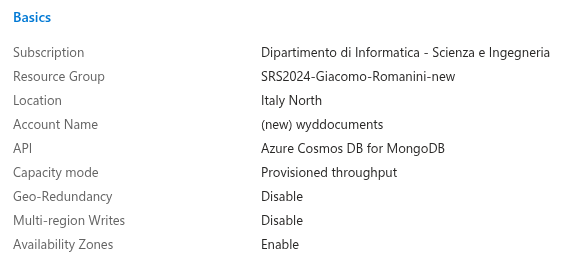
\includegraphics[width=\textwidth]{cosmosbasics.png}
    \caption{Impostazioni generali di Azure Cosmos DB}
\end{figure}

Volendo inizialmente rimanere in una singola regione,
l'impostazione "Geo-Redundancy" non è stata abilitata.
Allo stesso modo le scritture su più regioni non sono state abilitate,
preferendo un approccio centralizzato.\\
\\
Come modello di costo Azure propone due modalità distinte: Serverless e Provisioned throughput.
Nella modalità serverless il servizio scala in base alle richieste,
e considerando quindi solo l'effettivo utilizzo di risorse richieste.
Adatto a carichi di richieste improvvisi e sbilanciati,
non supporta l'esecuzione su più regioni.
Il provisioned throughput invece richiede una previsione delle risorse necessarie,
per metterle a disposizione e farsi pagare di conseguenza, che siano state usate o meno.
Questo necessita quindi di una stima del carico previsto,
per poi impostare le risorse.
Azure propone però un metodo chiamato autoscale, 
che permette di modificare automaticamente (all'interno di un intervallo predefinito)
le risorse messe a disposizione in base al carico del momento,
per poi considerare il massimo valore raggiunto in quell'ora.
Questo permette di evitare l'implementazione di una strategia,
mantenendo comunque i costi legati al consumo effettivo delle risorse.
Prevedendo un carico di richieste non troppo elevato,
ma anche costante e poco variegato, 
e considerando un tempo di latenza minore e il supporto a regioni multiple,
si è scelta una strategia di pagamento di tipologia Provisioned throughput,
che verrà poi impostata per scalare automaticamente in un intervallo di risorse inizialmente contenuto.\\
\\
Per migliorare la sicurezza del database e garantire il controllo degli accessi
il database è stato inserito all'interno di una rete virtuale privata,
limitando l'accesso ai soli altri nodi che ne fanno parte,
isolandolo verso l'esterno.
Verranno quindi aggiunti alla rete solo i servizi che devono comunicare con Cosmos DB,
in particolare Azure Functions e il KeyVault(che contiene le chiavi per la cifratura dei dati).
Nonostante la ridondanza nelle zone garantisca il ritrovamento dei dati 
anche in caso di indisponibilità di un'istanza del database,
si è scoperti qualora avvengano modifiche erronee o malintenzionate.
Il servizio di backup proposto da Azure permette di salvare lo stato dei dati 
fino a un certo momento nel passato, 
in maniera tale garantire il ritorno a una situazione precedente 
in caso ci si accorga siano avvenute modifiche non desiderate. 
Azure permette sia di personalizzare la tipologia di backup,
in termini di durata, grandezza dei salvataggi e numero di copie,
sia di seguire delle opzioni già configurate.
Nel nostro caso si è scelto di applicare il servizio incluso gratuitamente
che mantiene le modifiche avvenute negli ultimi sette giorni.\\


\subsection{La definizione delle collezioni}

Stabilita la tipologia e il comportamento del servizio che ospita il database, 
bisogna definire la struttura delle classi in maniera da sfruttare al meglio le sue proprietà,
allineando i dati alle procedure di lettura e scrittura,
per ottimizzare il carico e il tempo di risposta.\\
\\
Grazie alle proprietà di accoppiamento debole e al supporto alla denormalizzazione delle entità,
la libertà di modellazione del dominio fornita da Cosmos DB è massima. 
Partendo dalle entità principali, per ognuna di esse è stata associata una collezione.
Sono state così definite quindi le entità di User, Profile, Event, Image e Group, 
che rispondono agli omonimi elementi del dominio.
A Event e Profile si aggiungono ProfileDetails ed EventDetails,
che contengono i dati particolari di questi elementi.
Gli Account sono gestiti internamente da Firebase Authentication, 
e la loro relazione con gli utenti è stata mappata in un insieme all'interno di User 
tramite i loro Uid.
Allo stesso modo, laddove siano presenti relazioni uno a molti con cardinalità contenute,
è stato possibile integrare le relazioni all'interno degli oggetti stessi, duplicando i collegamenti.
È il caso delle immagini, in cui viene salvato il riferimento dell'Event in Image,
o di User e Profile, i quali contengono entrambi i corrispettivi riferimenti.
UserRole è stato integrato solo in ProfileDetails, 
essendo necessario per controllare i permessi di un utente verso un profilo, e non il contrario.\\
\\
La relazione tra profili e gruppi vede cardinalità elevate, 
infatti non è posto un limite al numero di gruppi a cui un profilo può fare parte.
Non richiedendo però dettagli particolari o interazioni complicate (in questa fase del progetto),
è stato considerato sufficiente mappare le relazioni tramite liste all'interno di Group e ProfileDetails.\\
\\
Come analizzato nelle sezioni precedenti, 
le richieste del progetto vertono sulla relazione tra eventi e profili.
In particolare, le richieste che sono previste più frequenti e quindi impattanti 
sono quelle di recupero dei dati generali delle entità su entrambi i versi della relazione
(eventi relativi ai profili o profili collegati agli eventi), 
ma anche di conferma di un evento.
Per prima cosa, vista la centralità di queste richieste,
sono state separate le proprietà essenziali da quelle di dettaglio,
salvandole in ProfileDetails ed EventDetails.
Questo permette di ridurre la mole di dati da recuperare e analizzare, 
rendendo le query meno pesanti e più veloci.
Questo migliora il tempo e la dimensione delle risposte per questo tipo di richieste, 
bilanciando il carico introdotto con le richieste aggiuntive derivate dalla separazione dell'entità.
Prevedendo richieste di conferma sullo stesso evento molto vicine tra loro
si è deciso di non integrare la relazione nelle entità esistenti, 
bensì di esternarla in documenti dedicati, 
per evitare modifiche concorrenti sullo stesso Event.\\
\\
\begin{figure}[htbp]
    \centering
    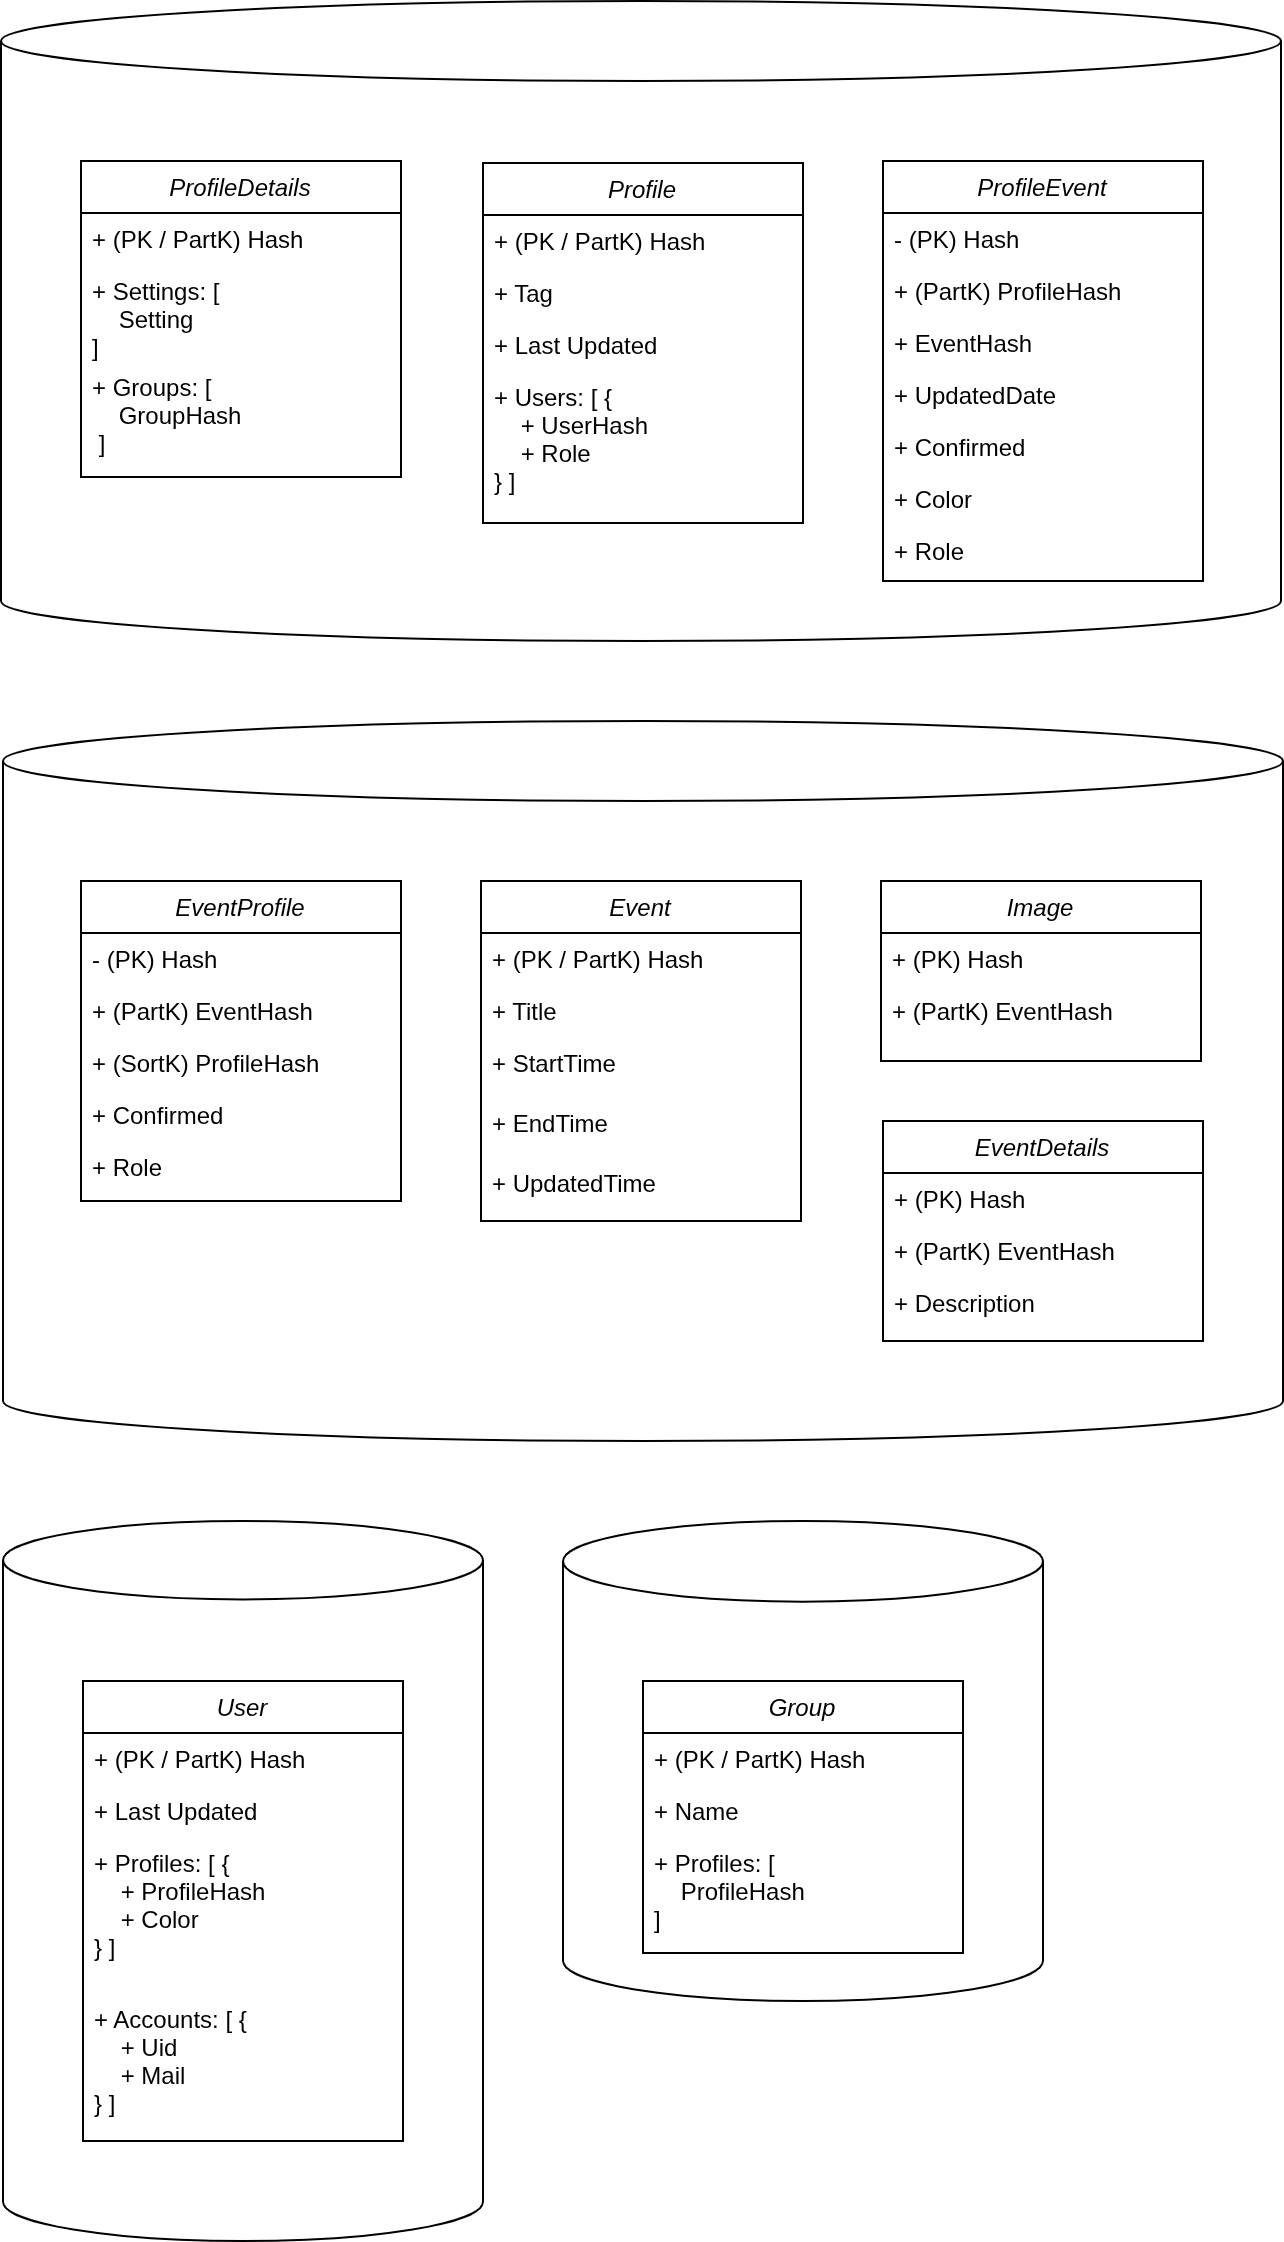
\includegraphics[height=.96\textheight]{NonRelazionalModel.png}
    \caption{Modello delle collezioni e il loro partizionamento}
\end{figure}
Si introduce così ProfileEvent, 
che presenta tutte le proprietà della relazione tra i due elementi. 
Venendo partizionato in base all'hash del profilo corrispondente,
assolve il compito di recuperare gli eventi associati al profilo.
Include quindi il collegamento all'evento e
la conferma o meno della partecipazione del profilo all'evento, 
ma anche la data dell'ultimo aggiornamento del profilo associato,
in maniera tale da consentire di controllare direttamente 
se un evento è stato modificato rispetto all'ultimo aggiornamento,
e deve quindi essere caricato.
Prevedendo però che la quantità di richieste sia comunque importante 
anche per ottenere dal lato opposto, 
ovvero ottenere i profili correlati agli eventi, 
non si può accettare una ricerca che attraversi le partizioni per recuperare queste informazioni.
Per questo motivo viene creato EventProfile, 
partizionato assieme agli eventi,
che mantiene le informazioni minime necessarie per mostrare i profili collegati, 
in maniera da limitare la quantità di dati da mantenere consistente.\\
\\
Analizzando questa relazione si evince che 
i campi replicati sono UpdatedDate e Confirmed.
nel momento in cui qualcuno modifica un campo principale dell'evento sarà necessario aggiornare tutte le istanze di ProfileEvent.
allo stesso modo, quando un profilo conferma la sua partecipazione ProfileEvent viene aggiornato, 
ma anche EventProfile deve ricevere la modifica.

\subsection{L'integrazione con le Azure Functions nel framework .Net}
L'utilizzo di un database documentale comporta un sviluppi implementativi specifici.
Il polimorfismo dei documenti e la denormalizzazione delle entità
rendono la rappresentazione logica degli elementi e la loro relazione reciproca di secondaria importanza.
L'approccio a oggetti del Framework .Net assume quindi minore rilevanza,
in quanto si rende meno necessaria la capacità di descrivere e astrarre 
le entità logiche attraverso classi di codice.
Si distinguono però due tipologie di richieste principali, 
che determinano l'approccio apportato verso i dati:
la recupera di un elemento e la sua modifica.\\
\\
Quando è necessario recuperare un elemento dal database risulta comodo 
convertirlo in un oggetto.
Questo consente di gestire le informazioni attraverso un'astrazione logica, con tutti i vantaggi relativi.
La sua utilità risalta sopratutto nel caso in cui la lettura dell'elemento 
non ha il solo fine di essere restituito al richiedente,
ma deve venire analizzato per procedere con la logica applicativa.
La rappresentazione dei documenti in oggetti comporta infatti un codice più pulito e ordinato, 
interagendo con le proprietà e i metodi della classe, senza entrare nella complessità computazionale 
dell'elaborazione del documento. 
La conversione viene svolta automaticamente dal framework, 
e permette di associare ai dati il codice strettamente relativo, creando metodi appositi.
Ogni elemento del dominio avrà quindi una classe associata,
con tutti i campi previsti dal modello.
Il contesto logico così introdotto agevola l'interazione tra i servizi e gli oggetti,
riducendo la probabilità di errori e semplificandone l'individuazione.
Anche il testing viene favorito, dando la possibilità di analizzare il codice 
senza la necessità di interrogare il database o di simularlo.
Permette inoltre di automatizzare la conversione dei dati verso i DataTransferObject(DTO), 
necessari per uniformare le risposte verso i client, 
che contribuiscono a separare la logica di business da quella che gestisce la comunicazione.\\
\\
Nel caso la richiesta richieda invece la modifica di un elemento 
la conversione del documento in oggetto risulta poco efficiente.
La creazione di un nuovo oggetto comporta infatti l'intera lettura dell'elemento associato.
Questo può essere utile se è necessario mantenere un riferimento logico,
se si useranno le informazioni che contiene
o se bisognerà restituire al mittente l'oggetto aggiornato.
Nella maggior parte dei casi invece si vuole semplicemente applicare una modifica,
lasciando che sia il sistema a propagarla.
In tal caso, Cosmos DB permette le cosiddette patch update, 
ovvero modifiche limitate al campo interessato,
senza richiedere la lettura e la sovrascrittura dell'intero documento.
Per queste occasioni vengono implementati appositi metodi che, 
preso in ingresso i dati da modificare, 
interagiscono con il database per aggiornare le sole parti coinvolte.\\
\\
La comunicazione con il database viene astratta tramite un servizio dedicato chiamato WydDbService.
WydDbService ha il compito di gestire le richieste e le sessioni con il database,
nascondendo le complessità implementative e di interazione.
In particolare, la connessione con il database comporta 
la richiesta verso Azure Key Vault per il recupero delle chiavi di accesso,
per poi usarle per stabilire un canale attraverso il quale applicare le modifiche. 
Mette inoltre a disposizione un'interfaccia per nascondere 
tutte le logiche di basso livello dovute dall'interazione specifica di CosmosDB.
Verrà utilizzato dagli altri servizi tramite dependency injection, 
automatizzandone la creazione e l'utilizzo, e di conseguenza la connessione e le richieste al database. \\

\subsection{Garantire la consistenza eventuale dei dati}

Avendo salvato le entità del dominio sotto forma di documenti denormalizzati
la modifica del campo di un elemento potrebbe dover comportare la necessità
di propagare gli aggiornamenti su tutti gli altri componenti in cui tale dato è duplicato.\\
\\
Potendo accettare un ritardo nell'allineamento dei dati,
affidare il compito di aggiornare tutti i componenti secondari coinvolti
alla stessa funzione che ha applicato i cambiamenti richiesti sul documento principale
risulta svantaggioso sotto molti aspetti.
Si introdurrebbe infatti un ritardo nell'esecuzione, 
dovuto all'attesa dell'applicazione delle ulteriori modifiche, 
che devono essere controllate e gestite in caso falliscano.
Complicare la funzione va inoltre contro i principi stessi 
dei servizi serverless, 
che prevedono invece strutture semplici con responsabilità precise e limitate.
La loro efficienza deriva infatti dalla possibilità 
di eseguire in maniera autonoma compiti specifici.
L'unico requisito necessario per permettere a una funzione di delegare ad altre le modifiche derivate
è la garanzia che la loro esecuzione venga controllata e quindi il loro successo sia assicurato.\\
\\
L'introduzione di una funzione con il ruolo di orchestratore 
non sposterebbe di molto il problema.
Per quanto soddisfi la necessità di suddividere il problema in diverse parti
per poi affidarle a diverse funzioni e sia in grado di controllarne il risultato, 
garantendone così il successo,
implica comunque il ritardo dovuto all'attesa del completamento delle funzioni, 
a cui va ad aggiungersi il tempo necessario per la sua stessa esecuzione,
influenzato dall'accoppiamento debole con le funzioni che chiama.
Si introdurrebbero inoltre dipendenze tra la funzione originale e
quelle derivate dalla modifica, che, non essendo necessarie, 
comportano solo rischi di fallimento e l'allungamento dei tempi di risposta.\\
\\
A questo scopo, Azure Cosmos DB mette a disposizione uno strumento apposito, chiamato Change Feed.
Change Feed è un meccanismo tramite il quale è possibile 
associare le modifiche di un elemento del database 
all'esecuzione di una funzione.
Il Change Feed viene definito come trigger all'interno di una funzione, 
e viene associato a una collezione di documenti.
Ogni volta che un documento di questa collezione subisce un aggiornamento
si crea in automatico un log che,
all'interno della partizione coinvolta, 
viene salvato in una nuova collezione dedicata chiamata "lease".
Il Change Feed è dunque un meccanismo che,
nel momento in cui un log viene aggiunto alla sua lease,
fa partire autonomamente la funzione associata.\\
\\
Una volta invocata, 
la funzione legge dal lease tutti i log che non sono ancora stati processati
per poi propagare le modifiche ove necessario.
L'avvenuta consegna ed elaborazione del log è registrata grazie a dei token di aggiornamento, 
che permettono di sapere in quale punto del lease sono presenti i log che non sono ancora stati processati.
La persistenza dei log sui lease consente di garantire 
che la modifica sia presa in carico da una funzione almeno una volta,
mentre la presenza dei token di aggiornamento assicura 
che la funzione venga eseguita di nuovo in seguito a un errore o a un guasto del sistema, 
soddisfando così i requisiti di invocazione.
Questo meccanismo è inoltre intrinsecamente scalabile. 
Essendo infatti i lease associati alle partizioni in cui risiedono i documenti,
è possibile dividere (e quindi distribuire, quando necessario) il carico su più funzioni.\\
\\
Il Change Feed viene usato, ad esempio, 
nel caso in cui venga cambiata un'informazione importante di un evento.
Questa operazione comporta l'aggiornamento di UpdatedDate, 
campo che memorizza il momento in cui è stata apportata l'ultima modifica.
UpdatedDate è stata denormalizzata all'interno dei ProfileEvent,
e la sua modifica deve essere quindi propagata.
Verrà quindi creata una funzione la cui invocazione sarà associata
alla presenza di log non elaborati nel lease relativo alla collezione degli Event.
In questa maniera i compiti vengono efficacemente suddivisi in due funzioni,
indipendenti tra loro.
La prima funzione avrà il solo compito di cambiare la proprietà dell'oggetto,
informando il client riguardo al successo dell'operazione.
Una seconda funzione, attivata in autonomia dal Change Feed, 
si occuperà poi di aggiornare di conseguenza tutti i ProfileDetails relativi,
senza andare a impattare sulle prestazioni o sulle dipendenze della prima.\\
\\
Ci sono situazioni in cui però il Change Feed non può essere usato.
È ad esempio il caso della conferma di un evento.
L'elemento primario coinvolto in questa operazione è ProfileEvent, 
che sarà modificato dalla funzione iniziale.
La conferma di partecipazione a un evento da parte di un profilo 
conta però come modifica all'evento stesso, 
che comporta quindi l'aggiornamento del documento Event.
Se si associasse però una funzione anche per le modifiche a ProfileEvent tramite Change Feed,
si verrebbe a creare una ricorsione infinita per il quale la modifica a un ProfileEvent 
comporta la modifica a un Event, che a sua volta comporta una modifica a ProfileEvent, e via dicendo.
Per quanto sia possibile aggiungere all'interno delle funzioni controlli 
che analizzino ogni volta l'origine della richiesta,
questo porterebbe a una maggiore complessità e carico implementativo,
introducendo nuovi dati all'interno di ogni aggiornamento. 
Si è quindi deciso di utilizzare il ChangeFeed solo per le entità 
la cui modifica influenza molteplici altri documenti,
delegando in maniera differente l'eventuale aggiornamento  richiesto di un singolo altro elemento.\\
\\
Ci sono diversi modi che le Azure Functions possono sfruttare 
per invocare un'altra funzione, senza passare per l'utilizzo di un orchestratore.
Una prima soluzione può essere l'invio di una nuova richiesta HTTP al server stesso,
al quale è associata la funzione voluta.
Per quanto risulti veloce e facile da implementare,
questa soluzione non garantisce però l'effettiva presa in carico, esecuzione e completamento della richiesta,
a meno di aspettarne la risposta per poi controllarla,
procedimento che minerebbe la finalità stessa dell'operazione.
Azure mette invece a disposizione servizi basati su code ed eventi 
proprio per mettere in comunicazione diverse parti di uno stesso sistema. 
Tra le funzionalità offerte da Azure e 
quindi direttamente integrabili con le Azure Functions troviamo 
Azure Queue Storage, Azure Service Bus e Azure Event Hub.\\
\\
Azure Queue Storage è un servizio di code di messaggi
offerto come parte di Azure Storage, 
che si occupa del salvataggio di informazioni 
che non rientrano nei casi d'uso dei database tradizionali.
Le funzioni hanno quindi la possibilità di aggiungere alla coda i propri messaggi,
che verranno poi elaborati da un'altra funzione grazie a un trigger associato.
La dimensione massima che i messaggi possono avere è di 64 KB,
e rimangono in memoria per un tempo prestabilito, che può essere configurato. 
Le code sono persistenti e altamente disponibili,
assicurando che i messaggi non vadano persi in caso di fallimento del consumer,
ma non presentano ulteriori funzionalità associate. 
La sua semantica di consegna garantisce che il messaggio venga elaborato almeno una volta,
il che significa che la sua consegna potrebbe avvenire più volte,
in caso di errori o di timeout di elaborazione da parte della prima funzione che lo ha preso in carico.
Presenta quindi un servizio semplice e veloce,
estremamente robusto ma anche scalabile.
La sua semplicità, sebbene contribuisca a ridurne il costo,
ne comporta però la mancanza di ulteriori proprietà avanzate.
Ad esempio, Azure Queue Service non presenta la capacità 
di gestire i messaggi in caso la loro esecuzione continui a fallire, 
che può essere desiderata in caso sia necessario assicurare che l'operazione giunga al suo termine.\\
\\
Azure Service Bus è invece un servizio di messaggistica
che supporta scenari più complessi rispetto a Queue Storage. 
Offre due tipologie principali di comunicazione: code e argomenti. 
Le code di Service Bus supportano le stesse funzionalità del servizio precedente,
a cui però se ne aggiungono di più avanzate quali l'ordinamento, 
le sessioni per il raggruppamento di messaggi correlati, 
la funzionalità di "dead-letter queue" integrata per la gestione automatica dei messaggi non elaborabili e 
l'elaborazione transazionale. 
Gli argomenti prevedono un pattern publish/subscribe,
nel quale più fruitori possono collegarsi allo stesso argomento per poi 
venire tutti notificati in contemporanea in caso venga inviato un messaggio a esso inerente.
Essendo stato progettato per soddisfare carichi di lavoro aziendale,
oltre a fornire garanzie di consegna più robuste e 
integrare meccanismi di gestione degli errori,
garantisce un'elevata scalabilità.
Risulta però più costoso e relativamente più complesso da utilizzare.\\
\\
Azure Event Hub è un servizio di ingestione di dati altamente scalabile e a bassa latenza, 
progettato per lo streaming di grandi volumi di eventi da diverse fonti. 
Non è una coda di messaggi nel senso tradizionale, 
ma piuttosto un "broker di eventi", 
in cui gli eventi vengono aggiunti a una coda distribuita su più partizioni 
dove rimangono disponibili per i consumer per un periodo configurabile (fino a 90 giorni). 
I consumer leggono gli eventi dalla partizione mantenendo ognuno il proprio progresso, 
il che permette a più consumer group di leggere gli stessi eventi indipendentemente. 
Anche in questo caso, la semantica garantisce che il messaggio venga elaborato almeno una volta.
Presenta quindi elevate caratteristiche di scalabilità, 
fornendo una bassa latenza, un throughput estremamente elevato
e la possibilità di parallelizzare il consumo dei messaggi.
Pur mantenendo in memoria i dati, 
e quindi assicurando che sia sempre possibile applicare le modifiche,
tutta la logica necessaria per controllare l'esecuzione, ritentare ed eliminare il messaggio 
rimane però a carico dello sviluppatore.\\
\\
\begin{longtable}{|P{2.9cm}|P{3.9cm}|P{3.9cm}|P{3.9cm}|}
    \hline
    \textbf{Caratteristica}&\textbf{Queue Storage}      & \textbf{Service Bus} & \textbf{Event Hub}\\
    \hline
    \endhead
    Tipo di servizio     & Coda di messaggi semplice   & Coda/Broker di messaggi & Flusso di eventi                               \\
    \hline
    Modalità di fruizione &  Competing Customers (Point-to-point) & Competing Customers (Point-to-point)\newline Publish/Subscribe (argomenti) & Publish/ Subscribe (molti a molti)                               \\
    \hline
    Caratteristiche & Semplice, scalabile e robusto ma nessun controllo degli errori & Affidabile, scalabile, garantisce e integra il controllo dell'esecuzione, ordinamento dei messaggi & Scalabile, robusto, ordinato ma nessun controllo sull'esecuzione\\
    \hline
    Costo & €0,04 GB/mese + €0.0004 ogni diecimila operazioni & €0,044 ogni milione di operazioni (piano Basic con solo le code)& €0,014/ora per ogni Unità di throughput + €0,025 ogni milione di eventi\\
    \hline
    \caption{Proprietà dei servizi Azure per la propagazione interna di messaggi }
\end{longtable}

Viste queste considerazioni, 
per garantire la consistenza degli oggetti nei casi in cui non sia possibile sfruttare il Change Feed
si è scelto di adottare Azure Service Bus.
La scelta deriva principalmente dalla suo supporto nativo al controllo dell'esecuzione delle funzioni,
grazie all'utilizzo di una dead-letter queue.
La dead-letter queue è un contenitore in cui vengono inseriti 
tutti i messaggi la cui elaborazione è fallita una determinata quantità di volte.
Garantisce quindi, in aggiunta a ulteriori tentativi in caso di insuccesso, 
il monitoraggio di tutte le operazioni che non riescono a essere portate a termine.
Questo permette di assicurare che gli aggiornamenti necessari per allineare i documenti
siano sempre controllati.\\
\\
Tornando all'esempio precedente, 
nel quale era necessario propagare la conferma di un evento, 
la modifica di Event e di EventProfile verrà eseguita da due funzioni dedicate.
Al termine della modifica di ProfileEvent, 
la funzione inserirà in coda al Service Bus un messaggio 
con le informazioni necessarie alle altre due,
per poi inviare la risposta al client.
Le due funzioni verranno quindi invocate, 
aggiornando gli elementi coinvolti.
Nel caso di Event, il Change Feed associato aggiornerà di conseguenza 
tutti i sui ProfileEvent, senza però creare ricorsioni.\\
\\
immagine interazione conferma\\
\\





\clearpage




La scelta di un database relazionale per la persistenza ha comportato sviluppi progettuali precisi.
In primis si rende necessario tradurre il dominio in componenti relazionali che possano essere espressi e salvati nelle tabelle del database.

var cosmosClient = new CosmosClient("<your-connection-string>");

per il collegamento da remoto, è necessario utilizzare una VPN per connettersi alla virtual Network

Si creano quindi sul server le classi logiche del programma, a partire dal dominio.
Ogni classe corrisponde ad un oggetto del dominio, presentando i valori e le relazioni dei componenti come attributi dell’oggetto.\\
\\
Una volta collegato il server con il database tramite le stringhe di connessione salvate sull’Azure Key Vault,
sono state definite le proprietà tra le varie entità, per poi inizializzare in automatico la struttura del database.
Le modifiche alla struttura del database vengono infatti generate automaticamente da EFCore in seguito alla creazione o alla modifica degli attributi degli oggetti.
Questo permette di star dietro agli aggiornamenti, generando e salvando le modifiche da applicare ad ogni modifica delle proprietà del dominio.\\
\\


Per la riduzione del carico computazionale richiesto da elementi con tante relazioni si utilizza la tecnica del lazy loading.
La tecnica del Lazy Loading consiste nel richiedere i dati delle relazioni di un elemento solo quando strettamente necessario.
La sua realizzazione tramite EFCore è attuata grazie alla proprietà virtual,
che permette di gestire un oggetto con un riferimento al database richiedendo i dati delle sue relazioni solo quando viene espressamente richiesto.\\
\\


Inoltre, Azure mette a disposizione molteplici servizi accessori che possono essere uniti al servizio.
Questo permette di estendere le potenzialità del database tramite  l’analisi e il monitoraggio dei dati,
generando prestazioni aggiuntive o integrando i dati per lo sviluppo di altre tecnologie.\\
\\

Al server principale è stata affiancata una replica che rimane costantemente aggiornata.
Situata in una località differente dal server principale,
garantisce alta disponibilità continuando a fornire i servizi anche in caso di malfunzionamenti al server principale.\\
\\

Nel caso in cui però fossero necessarie ulteriori prestazioni,
se il dominio e i requisiti lo permettono,
si può eventualmente delegare a un database non relazionale le modifiche ai dati e alle relazioni
che non necessitano delle qualità ACID ma richiedono un’alta frequenza di scrittura.\\
\\
Interporre una cache tra la logica applicativa e il database
semplifica e riduce il numero di richieste verso il database.
Il livello di caching si occupa di gestire le richieste al database
fornendo e duplicando le risposte che possiede già in memoria,
eventualmente concentrando le richieste in caso i dati siano invece da recuperare.
Per i dati in scrittura, invece, salva temporaneamente le modifiche richieste,
aggiornando subito la memoria locale,
per poi apportare le modifiche al database in momenti di carico ridotto.
Garantisce così un tempo di risposta e di propagazione degli aggiornamenti ridotto,
alleviando il numero di richieste al database, estendendo così  le prestazioni fornite.\\
\\


Tuttavia, non vi è alcun vincolo che impedisca l'affiancamento di database di tipologia diversa
per rispondere a esigenze specifiche e sfruttare i punti di forza di entrambe le tecnologie.
\\
\clearpage